\section{Глобулярные конформации}
Как уже говорилось, конформации при низких температурах переходит в глобулярную фазу. Данные конформации отличаются более плотно расположенными вершинами, большинство из которых имеет 4 или 3 соседа. Конформации данного вида предположительно имеют магнитные свойства, схожие с двумерной квадратной решёткой. 

Для вычислений были сгенерированы по 1000 конформаций длины 250, 500, 1000, 2000. При моделировании методом Монте-Карло делалось 10000--30000 шагов на отжиг, и 50000--100000 шагов для замеров. 
Оказалось что достаточно большая часть этих конформаций неплотные, то есть их свойства ближе к свойствам одномерной решётки, чем двумерной. При попытке посчитать среднее значения кумулянта Биндера неплотные конформации сильно влияли на значение кумулянта, увеличивая погрешность от реплики к реплике.

\begin{figure}[ht]
	\centering
	\begin{subfigure}[t]{0.48\textwidth}
		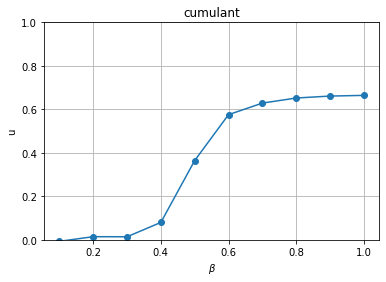
\includegraphics[width=\textwidth]{../images/dense_cumulant.png} 
		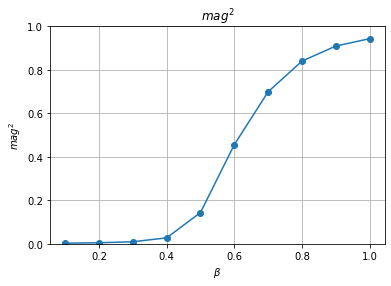
\includegraphics[width=\textwidth]{../images/dense_magnetization.png} 
		\caption{Плотная}
	\end{subfigure}
	\begin{subfigure}[t]{0.48\textwidth}
		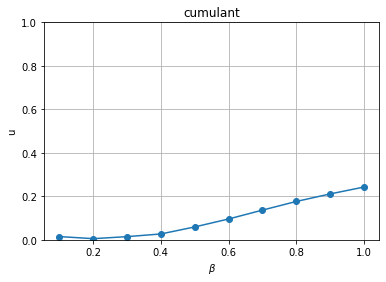
\includegraphics[width=\textwidth]{../images/loose_cumulant.png} 
		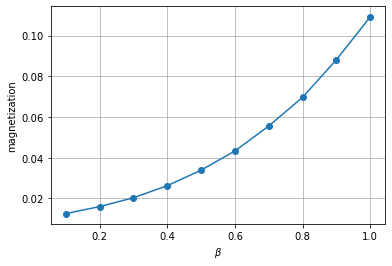
\includegraphics[width=\textwidth]{../images/loose_magnetization.png} 
		\caption{Неплотная}
	\end{subfigure}
	\caption{Пример кумулянта и намагниченности плотной и неплотной конформаций}
\end{figure}


\subsection{Разделение конформаций}

Для отделения плотных конформаций от остальных было предложено вычислять их радиус инерции. 
\[
R = \sqrt{\frac{1}{n}\sum_{i=1}^{n}r_{i}^{2}}
\]
где $r_i$ это расстояние от узла конформации до её центра масс. 

Однако при рассмотрении большого количества конформаций оказалось, что маленький радиус инерции не гарантирует хорошую намагниченность конформации. Это хорошо видно при рассмотрении намагниченности конформаций при низких температурах $\beta = 1$

\begin{figure}[ht]
	\centering
	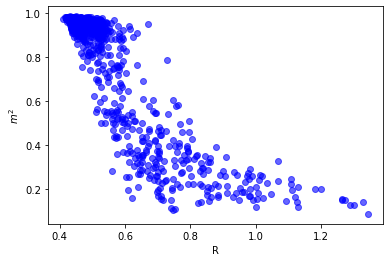
\includegraphics[width=0.5\textwidth]{../images/mag2_to_R_L250.png} 
	\caption{Квадрат намагниченности и радиус инерции конформаций длины $L = 250$ при $\beta = 1$}
	\label{fig:mag2_to_R} 
\end{figure}

На рис.\ref{fig:mag2_to_R}, при $R \approx 0.6$ $m^2$ принимают любые значения от $0.2$ до $1.0$. Значит, при разделении конформации только по радиусу инерции, мы либо будем отбрасывать намагничивающиеся конформации, либо оставлять не намагничивающиеся

\subsubsection*{Кластеризованные конформации.} \label{par:clusterized_conformations}


На искусственном примере рис.\ref{fig:synth_cluster_conf} показана одна из причин, по которой плотная конформация может плохо намагничиваться. Тут имеется несколько крупных двумерных кластеров, соединённых одномерной цепочкой. И несмотря на то, что сами по себе эти кластеры намагничиваются, направление спинов в них слабо связано, из-за чего спины в разных кластерах с большой вероятностью будут направлены в противоположные стороны. Далее соединяющие цепочки будут называться мостами, а длина моста - количество вершин, входящих в него.

\begin{figure}[ht]
	\centering
	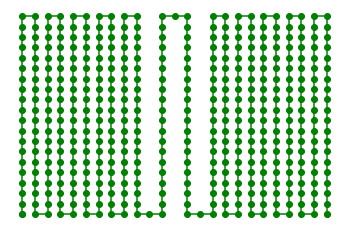
\includegraphics[width=0.47\textwidth]{../images/2Cluster_conformation.png}
	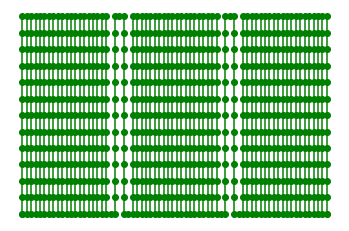
\includegraphics[width=0.47\textwidth]{../images/3Cluster_conformation.png} 
	\caption{Пример плотных немагнитных конформаций с двумя и тремя кластерами}
	\label{fig:synth_cluster_conf}
\end{figure}

На рис.\ref{fig:synth_cluster_conf} приведён пример с очень длинным мостом, чтобы показать, что конформации могут одновременно иметь малый радиус инерции и большую длину моста, однако даже в большинстве сгенерированных конформаций длины мостов оказываются значительно меньше.

Для лучшего понимания влияния размеров мостов и кластеров, и количества кластеров на магнитные свойства модели, мы рассмотрели искусственные модели конформаций с кластерами размером: 250, 500, 1000, 2000, количеством кластеров: 2, 3, 4, и длинами мостов между ними от 1 до 10. Кластеры в конформациях имеют прямоугольную форму и последовательно соединены мостами снизу. Пример конформаций представлен на рис. \ref{fig:cluster_conf_example}.

\begin{figure}[ht]
	\centering
	\includegraphics*[width=0.4\textwidth]{../images/3Cluster_conformation_short.png}
	\caption{Пример модели кластеризованной конформации с тремя кластерами и мостами длины 6.}
	\label{fig:cluster_conf_example}
\end{figure}

Абсолютные размеры кластеров не показали значительного влияния на магнитные свойства, поэтому далее будут рассматриваться конформации с кластерами размера 2000.

На рис. \ref{fig:cluster_magnetization} видно, что увеличение количества кластеров, и длины мостов ведёт к уменьшению магнитной восприимчивости. Так же можно сказать, что количество кластеров имеет большее влияние на намагниченность, чем длина мостов. А так как в данном случае количество кластеров напрямую связано с относительным размером кластера, то и относительный размер кластеров, оказывает большее влияние на магнитные свойства модели, чем длина мостов. Данное замечание будет важно далее, при разделении сгенерированных конформаций.

\begin{figure}[ht]
	\centering
    \begin{subfigure}[t]{0.45\textwidth}
        \includegraphics*[width=\textwidth]{../images/magnetization_clusterized_W20_H50_N2.png}
        \caption*{2 кластера}
    \end{subfigure}
    \begin{subfigure}[t]{0.45\textwidth}
        \includegraphics*[width=\textwidth]{../images/magnetization_clusterized_W20_H50_N3.png}
        \caption*{3 кластера}

    \end{subfigure}
    \begin{subfigure}[t]{0.45\textwidth}
        \includegraphics*[width=\textwidth]{../images/magnetization_clusterized_W20_H50_N4.png}
        \caption*{4 кластера}
    \end{subfigure}
	\caption{Квадрат намагниченность конформаций с кластерами размера 2000, цветами отмечена длина мостов между кластерами}
	\label{fig:cluster_magnetization}
\end{figure}


Было сделано предположение, что можно определять намагничивающиеся конформации используя кластеры и мосты. Следующей задачей стало проанализировать конформации на количество и размеры кластеров, а так же мостов. Однако пока мы не дали чёткого определения моста и кластера. Поэтому были рассмотрены несколько вариантов.

Первым вариантом было искать классические мосты -- спины, при удалении которых увеличивается число компонент связанности графа. Однако такой способ не дал желаемого эффекта, так как кластеры могут быть соединены более чем одним мостом. И например на конформации из рис. \ref{fig:clusters_and_bridges} данный способ не выделяет ни одного моста, хотя там очевидно есть структуры, отделённые друг от друга одномерными цепочками. 

Следующий алгоритм выделял как мосты все цепочки спинов у которых 1 или 2 соседа, однако при таком подходе мы получаем мосты, которые соединяют один и тот же кластер. Такие мосты не разделяют кластеры и не оказывают на конформацию эффект описанный выше. Так же этим способом мы выделяем множество вершин на краях конформации как мосты, например вершины в углах прямоугольника будут считаться мостами, что очевидно неправильно.

Итоговая версия алгоритма выделяет как мосты все спины, которые имеют 1 или 2 соседа, и затем добавляет мосты, которые соединяют один и тот же кластер, к этому же кластеру. Таким образом мы оставляем только мосты, разделяющие конформацию на отдельные плотные части, которые мы и называем кластерами. Данный алгоритм описан ниже.

\paragraph{Алгоритм разбиения на мосты и кластеры}
\begin{enumerate}
	\item Отмечаем все спины с 1 или 2 соседями как мосты.
	\item Создаём массив, где отмечаем посещённые спины. Создаём массив где для каждого спина будем писать номер его кластера. И переменную отвечающую за текущую длину моста $l$. Изначально все спины не посещены, $l = 0$.
	\item Начинаем идти по конформации от первой вершины.
	\begin{enumerate}
	
		\item Если спин отмечен как мост, то увеличиваем $l$ на 1
		\item Если спин не отмечен как мост и не посещён, увеличиваем счётчик кластеров на 1 и запускаем DFS(Алгоритм DFS описан ниже). Если $l > 0$ увеличиваем счётчик мостов на 1, длина нового моста $= l$. Обнуляем $l$
		\item Если спин не мост, уже посещён, последний встреченный спин, не являющийся мостом, принадлежит тому же кластеру и текущая длина моста $l > 0$. Значит этот мост соединяет один и тот же кластер. Поэтому добавляем предыдущие $l$ спинов к этому кластеру, обнуляем $l$.
		\item Если спин не мост, посещён, но номер кластера отличается от последнего встреченного кластера: если $l > 0$ увеличиваем счётчик мостов на 1, длина нового моста $= l$. Обнуляем $l$
	\end{enumerate}
	\item Проверяем первый и последний мост, если они соединяют один и тот же кластер, или один из их концов не соединён ни с каким кластером, добавляем их в кластер, с которым они соединены.
\end{enumerate}

\textbf{Алгоритм DFS}
\begin{enumerate}
	\item Заходим в вершину.
	\item Отмечаем вершину как посещённую.
	\item Отмечаем номер её кластера.
	\item Увеличиваем счётчик размера текущего кластера на 1.
	\item Заходим во все соседние непосещённые вершины не мосты.
\end{enumerate}

В данном алгоритме мы пользуемся тем, что мосты обязательно образуются из подряд идущих вершин конформации. Поэтому чтобы определить соединяет ли мост один и тот же кластер, нам достаточно, идя по конформации, запоминать последний встреченный кластер и сравнивать его с новым.
Результатом работы алгоритма являются размеры кластеров и мостов в конформации, а так же для каждой вершины однозначно определяется кластер или мост, которому она принадлежит. Пример работы алгоритма представлен на рис. \ref{fig:clusters_and_bridges}, данная конформация так же является примером того, как глобулярная конформация с малым радиусом инерции может оказаться разбитой на кластеры, и из-за этого слабо намагничиваться.

\begin{figure}[ht]
	\centering
	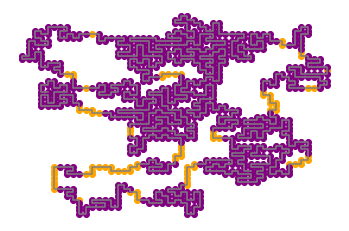
\includegraphics[width=0.70\textwidth]{../images/bridges_example_1.png}  
	\caption{Пример реальных конформаций с маленьким радиусом инерции и маленькой намагниченностью. Фиолетовым отмечены кластеры, жёлтым -- мосты}
	\label{fig:clusters_and_bridges}
\end{figure}

\subsection{Статистика по кластерам и мостам}
Ниже представлены гистограммы с размерами и числом кластеров и мостов в конформациях. Посчитано на 10000 конформациях с длинами 250, 500, 10000, конформации получены при $\frac{U}{T} = 1$. Размеры кластеров и длины мостов нормированы на длины конформаций. 


\begin{figure}[H]
	\centering
	\begin{subfigure}[t]{0.3\textwidth} 
		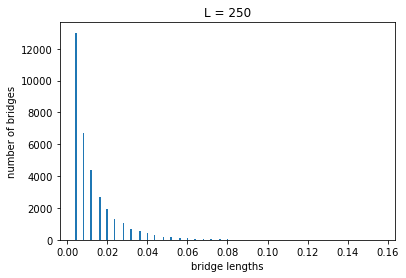
\includegraphics[width=\textwidth]{../images/bridge_lengths_L250.png} 
	\end{subfigure}
	\begin{subfigure}[t]{0.3\textwidth} 
		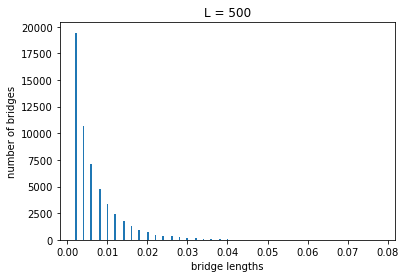
\includegraphics[width=\textwidth]{../images/bridge_lengths_L500.png} 
	\end{subfigure}
	\begin{subfigure}[t]{0.3\textwidth} 
		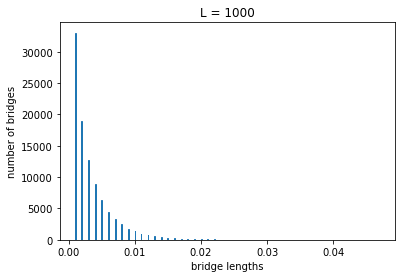
\includegraphics[width=\textwidth]{../images/bridge_lengths_L1000.png} 
	\end{subfigure}
	\caption{Распределение длин мостов.}
\end{figure}

\begin{figure}[H]
	\centering
	\begin{subfigure}[t]{0.3\textwidth} 
		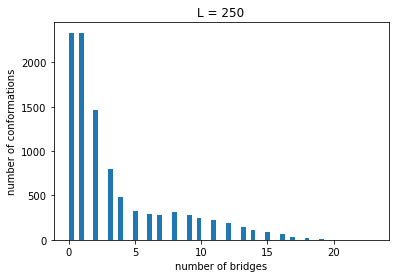
\includegraphics[width=\textwidth]{../images/bridges_count_L250.png} 
	\end{subfigure}
	\begin{subfigure}[t]{0.3\textwidth} 
		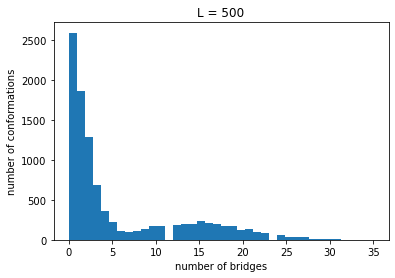
\includegraphics[width=\textwidth]{../images/bridges_count_L500.png} 
	\end{subfigure}
	\begin{subfigure}[t]{0.3\textwidth} 
		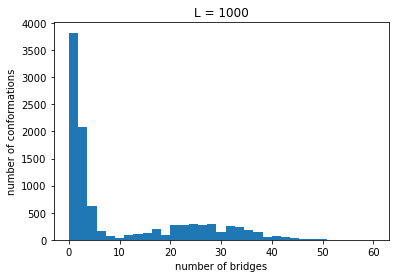
\includegraphics[width=\textwidth]{../images/bridges_count_L1000.png} 
	\end{subfigure}
	\caption{Распределение числа мостов в конформации.}
\end{figure}

\begin{figure}[H]
	\centering
	\begin{subfigure}[t]{0.3\textwidth} 
		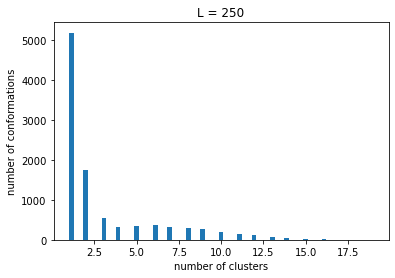
\includegraphics[width=\textwidth]{../images/clusters_count_L250.png} 
	\end{subfigure}
	\begin{subfigure}[t]{0.3\textwidth} 
		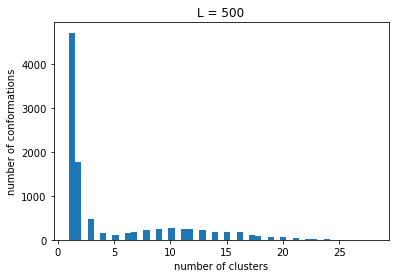
\includegraphics[width=\textwidth]{../images/clusters_count_L500.png} 
	\end{subfigure}
	\begin{subfigure}[t]{0.3\textwidth} 
		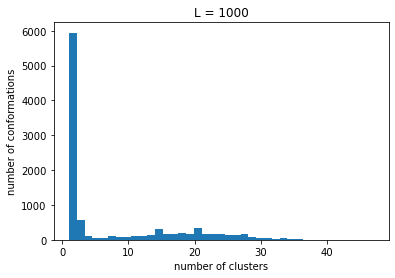
\includegraphics[width=\textwidth]{../images/clusters_count_L1000.png} 
	\end{subfigure}
	\caption{Распределение числа кластеров в конформации.}
\end{figure}

\begin{figure}[H]
	\centering
	\begin{subfigure}[t]{0.3\textwidth} 
		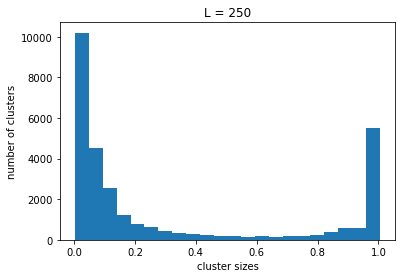
\includegraphics[width=\textwidth]{../images/cluster_sizes_L250.png} 
	\end{subfigure}
	\begin{subfigure}[t]{0.3\textwidth} 
		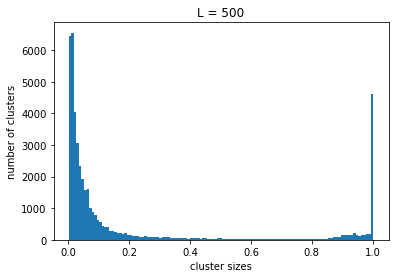
\includegraphics[width=\textwidth]{../images/cluster_sizes_L500.png} 
	\end{subfigure}
	\begin{subfigure}[t]{0.3\textwidth} 
		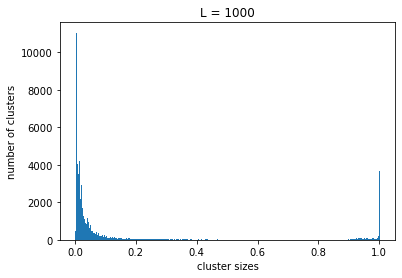
\includegraphics[width=\textwidth]{../images/cluster_sizes_L1000.png} 
	\end{subfigure}
	\caption{Распределение размера кластеров.}
\end{figure}

\begin{figure}[H]
	\centering
	\begin{subfigure}[t]{0.3\textwidth} 
		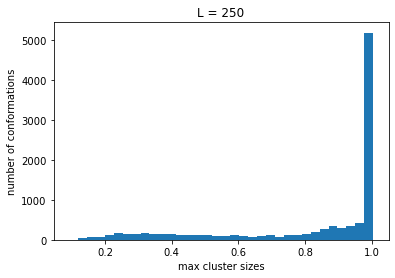
\includegraphics[width=\textwidth]{../images/max_cluster_size_L250.png} 
	\end{subfigure}
	\begin{subfigure}[t]{0.3\textwidth} 
		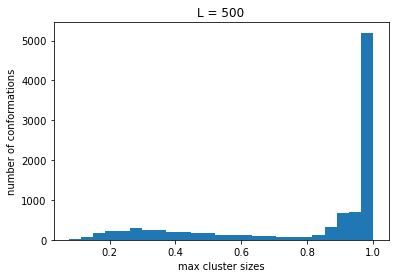
\includegraphics[width=\textwidth]{../images/max_cluster_size_L500.png} 
	\end{subfigure}
	\begin{subfigure}[t]{0.3\textwidth} 
		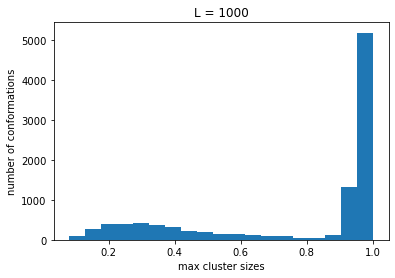
\includegraphics[width=\textwidth]{../images/max_cluster_size_L1000.png} 
	\end{subfigure}
	\caption{Распределение размера наибольшего кластера в конформации.}
\end{figure}


\subsection{Результаты разбиения на кластеры}
Результаты анализа связи между намагниченностью и количеством и размерами кластеров и мостов подтверждают сказанное выше. У конформаций с большим числом кластеров обычно намагниченность ниже чем у конформаций с одним большим кластером. 

Были рассмотрены несколько параметров: количество мостов, количество кластеров, суммарная длина мостов, размер наибольшего кластера. Наилучшим способом разделения конформаций на магнитные и немагнитные сейчас выглядит именно разделение по размеру наибольшего кластера. Как видно на рис.\ref{fig:mag_from_max_cluster} при разбиении по данному параметру разброс намагниченности значительно ниже, чем при разбиении по радиусу инерции. Данный параметр можно легко масштабировать для разных длин конформаций.

\begin{figure}[ht]
	\centering
	\caption{График размера наибольшего кластера и квадрата намагниченности для 10000 конформаций длины 1000}
	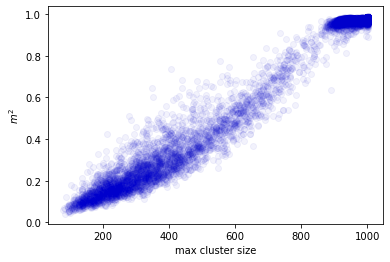
\includegraphics[width=0.6\textwidth]{../images/mag_from_cluster_size.png} 
	\label{fig:mag_from_max_cluster}
\end{figure}

\subsubsection*{Сравнение разделения по кластерам и по радиусу}
Чтобы оценить и сравнить эффективность разбиения конформаций при помощи размера наибольшего кластера и радиуса инерции воспользуемся следующим способом.

\begin{enumerate}
	\item Зададим значение намагниченности $\mu$, начиная с которого будем считать конформации намагниченными.
	\item Из всех сгенерированных конформаций возьмём $n$ конформаций с наименьшими радиусом инерции, и $n$ конформаций с наибольшими размерами кластеров.
	\item Среди выбранных конформаций посчитаем $k_{\mu, n}$ -- количество конформаций, намагниченность которых $< \mu$. Чем ниже это значение, тем лучше соответствующий способ разделения.
	\item Повторяем предыдущие пункты для разных значений $\mu$ и $n$.
\end{enumerate}

Сравнивая полученные значения $k_{\mu, n}$, можем определить, какой из способов эффективнее. На рис.\ref{fig:kmun_example} видно как примерно ведут себя данные значения: до определённого n они равны 0, затем, дойдя до границы между магнитными и немагнитными конформациями, оно начинает расти, после чего рост становится линейным, так как все оставшиеся конформации не являются магнитными. 
Лучше разницу между двумя способами видно на рис.\ref{fig:kmun_dif}, где, при всех значениях $\mu$ и $n$ разница $k_{\mu, n}$ остаётся отрицательной. То есть разделения по радиусу инерции всегда оставляет больше немагнитных конформаций, чем разделение по размеру кластеров.

\begin{figure}[H]
	\centering
	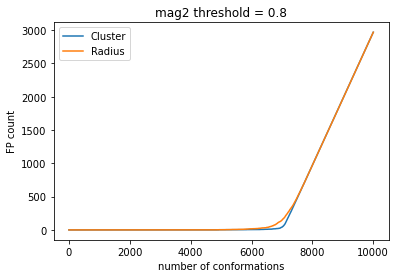
\includegraphics[width=0.6\textwidth]{../images/cluster_and_radius_mu0.8.png} 
	\caption{График $k_{\mu, n}$ для разделения по кластерам и по радиусу при $\mu = 0.8$.}
	\label{fig:kmun_example}
\end{figure}

\begin{figure}[H]
	\centering
	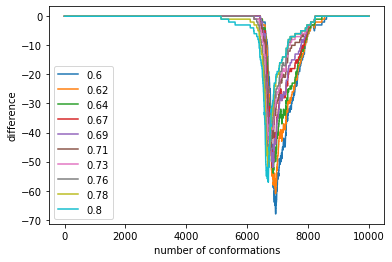
\includegraphics[width=0.6\textwidth]{../images/radius_and_cluster_comparising_L1000.png}
	\caption{График разности: $k_{\mu, n}$ при кластерном разделении и $k_{\mu, n}$ при разделении по радиусам. На 10000 конформаций длины 1000. Каждая линия соответствует одному значению $\mu$.}
	\label{fig:kmun_dif}
\end{figure}



\subsection{Кумулянт и точка перехода}

Кумулянт Биндера для одной реплики при заданной температуре вычисляется по формуле 
\[
U = 1 - \frac{\langle m^4\rangle}{3\langle m^2\rangle ^2}
\]
Дальше Значения усредняются между репликами при каждой температуре 
\[
\langle U\rangle = \frac{1}{n}\sum_{i=1}^{n}U_i
\]
Погрешность кумулянта от реплики к реплике вычисляется как среднеквадратичное отклонение по формуле 
\[
\sqrt{\frac{1}{n}\sum_{i=1}^{n}(\langle U\rangle - U_i)^2}
\]

Как видно на рис.\ref{fig:cumulant_raw}, вычисление кумулянта на всех сгенерированных конформациях даёт слишком большие погрешности от конформации к конформации, из-за этого становится невозможно определить точку перехода.

\begin{figure}[ht]
	\centering
	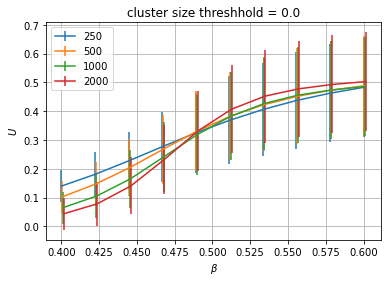
\includegraphics[width=0.5\textwidth]{../images/Cumulant_raw_beta0.4_0.6.png}
	\caption{кумулянты построенные на всех полученных конформациях}
	\label{fig:cumulant_raw}
\end{figure}

Описанный выше способ разделения конформаций на магнитные и немагнитные должен позволить уменьшить погрешность при вычислении кумулянта. Чтобы подобрать значение параметра (размер наибольшего кластера), при котором будет происходить разделение, мы стали перебирать значения, и следить за поведением точки пересечения. Предположительно при увеличении параметра точка пересечения должна двигаться в сторону нуля, и, начиная с определённого значения она должна остановиться.

Так как погрешность при вычислении кумулянта всё равно остаётся достаточно большой, мы используем следующий подход для вычисления точки пересечения. Рядом с предполагаемой точкой пересечения берём несколько соседних значений $\beta$, в которых мы делали замеры. Используя среднее значение и среднеквадратичное отклонение кумулянта для конформаций в этих точках как параметры для нормального распределения, генерируем новые значения кумулянта. Далее, используя метод наименьших квадратов, проводим отрезок наиболее близкий к сгенерированным точкам. Таким образом генерируем пары отрезков для конформаций разных длин, определяем точки пересечения каждой пары отрезков (если отрезки не пересекаются, генерируем заново), и затем усредняем координаты пересечений.

Мы рассмотрели различные значения минимального размера кластера, начиная с которого мы будем использовать конформации для вычисления кумулянта. Как и ожидалось, при увеличении размера кластера, ожидаемая точка пересечения сдвигается в сторону нуля, и в какой-то момент останавливается.

\begin{figure}[ht]
	\centering
	\begin{subfigure}[t]{0.3\textwidth}
		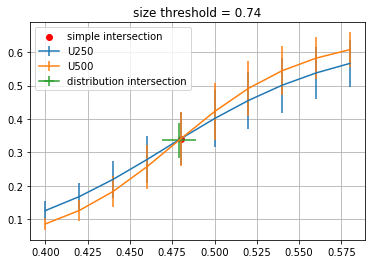
\includegraphics[width=\textwidth]{clusters_cumulant_3pts_dist.png}
		\caption{распределение по 3 точкам}
	\end{subfigure}
	\begin{subfigure}[t]{0.3\textwidth}
		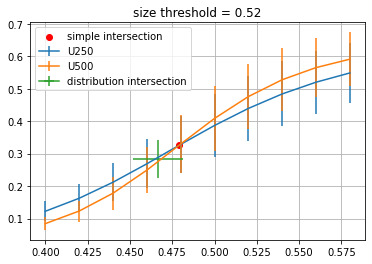
\includegraphics[width=\textwidth]{clusters_cumulant_4pts_thr=0.52.png}
		\caption{распределение по 4 точкам справа}
	\end{subfigure}
	\begin{subfigure}[t]{0.3\textwidth}
		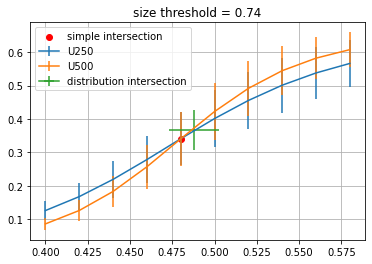
\includegraphics[width=\textwidth]{clusters_cumulant_4pts_thr=0.74.png}
		\caption{распределение по 4 точкам слева}
	\end{subfigure}
	\caption{Точки пересечения, полученные после разделения конформация по размеру кластерав, полученные генерацией отрезков с использованием разных точек замеров.}
	\label{fig:ditrib_intersection}
\end{figure}

Однако несмотря на уменьшение погрешности, она всё ешё слишком большая для точного определения точки перехода. На рис. \ref*{fig:ditrib_intersection} приведены примеры полученных точек пересечения. Из-за больших погрешностей кумулянта, сгенерированные точки пересечения очень сильно зависят от того, какие точки мы возьмём для генерации. При изменении минимального требуемого размера кластера результат почти не меняется. 

Пока что мы не нашли способа точно определить точку перехода, используя кумулянт Биндера, из-за того что даже среди глобулярных конформаций значения намагниченности имеют слишком большой разброс, что приводит к большим погрешностям кумулянта. Дальнейшие попытки определить точку перехода будут опираться на другие методы.